\documentclass{article}
\usepackage[utf8x]{inputenc}
\usepackage{ucs}
\usepackage{amsmath} 
\usepackage{amsfonts}
\usepackage{marvosym}
\usepackage{wasysym}
\usepackage{upgreek}
\usepackage[english,russian]{babel}
\usepackage{graphicx}
\usepackage{float}
\usepackage{textcomp}
\usepackage{hyperref}
\usepackage{geometry}
  \geometry{left=2cm}
  \geometry{right=1.5cm}
  \geometry{top=1cm}
  \geometry{bottom=2cm}
\usepackage{tikz}
\usepackage{ccaption}
\usepackage{multicol}

\hypersetup{
   colorlinks=true,
   citecolor=blue,
   linkcolor=black,
   urlcolor=blue
}

\usepackage{listings}
%\setlength{\columnsep}{1.5cm}
%\setlength{\columnseprule}{0.2pt}

\usepackage[absolute]{textpos}

\renewcommand{\thesubsection}{\arabic{subsection}}

\begin{document}
\pagenumbering{gobble}
\lstset{
  language=C,                % choose the language of the code
  basicstyle=\linespread{1.1}\ttfamily,
  columns=fixed,
  fontadjust=true,
  basewidth=0.5em,
  keywordstyle=\color{blue}\bfseries,
  commentstyle=\color{gray},
  stringstyle=\ttfamily\color{orange!50!black},
  showstringspaces=false,
  numbersep=5pt,
  numberstyle=\tiny\color{black},
  numberfirstline=true,
  stepnumber=1,                   % the step between two line-numbers.        
  numbersep=10pt,                  % how far the line-numbers are from the code
  backgroundcolor=\color{white},  % choose the background color. You must add \usepackage{color}
  showstringspaces=false,         % underline spaces within strings
  captionpos=b,                   % sets the caption-position to bottom
  breaklines=true,                % sets automatic line breaking
  breakatwhitespace=true,         % sets if automatic breaks should only happen at whitespace
  xleftmargin=.2in,
  extendedchars=\true,
  keepspaces = true,
}
\lstset{literate=%
   *{0}{{{\color{red!20!violet}0}}}1
    {1}{{{\color{red!20!violet}1}}}1
    {2}{{{\color{red!20!violet}2}}}1
    {3}{{{\color{red!20!violet}3}}}1
    {4}{{{\color{red!20!violet}4}}}1
    {5}{{{\color{red!20!violet}5}}}1
    {6}{{{\color{red!20!violet}6}}}1
    {7}{{{\color{red!20!violet}7}}}1
    {8}{{{\color{red!20!violet}8}}}1
    {9}{{{\color{red!20!violet}9}}}1
}

\title{Семинар \#5: Структуры. Домашнее задание.\vspace{-5ex}}\date{}\maketitle
В задачах потребуются исходный код и входные файлы, которые можно найти по адресу: \\
\href{https://github.com/v-biryukov/cs_mipt_faki/tree/master/term1/seminar05_struct/homework/files}{github.com/v-biryukov/cs\_mipt\_faki/tree/master/term1/seminar05\_struct/homework/files}


\section*{Структура Актёр (\texttt{Actor})}

\begin{lstlisting}
struct actor
{
	char name[32];
	char surname[32];
	int gender;
	int height;
	Date birth_date;
	Address birth_address;
};
typedef struct actor Actor;
\end{lstlisting}

Поля структуры \texttt{Actor}:
\begin{itemize}
\item \texttt{name} -- имя актёра
\item \texttt{surname} -- фамилия
\item \texttt{gender} -- пол (\texttt{0}, если это мужчина; \texttt{1}, если это женщина)
\item \texttt{height} -- рост в сантиметрах
\item \texttt{birth\_date} -- дата рождения (структура, содержащая 3 числа)
\item \texttt{birth\_address} -- место рождения (структура, содержащая 3 строки: страна, регион и город)
\end{itemize}


\subsection*{Файл \texttt{actors.csv}:}
В файле \texttt{actors.csv} содержится информация о 2000 актёрах (все данные сгенерированы случайным образом). Файл имеет следующий вид:
\begin{verbatim}
2000
Abel,Garifullin,0,189,16/2/1992,Russia,Rostovskaya Oblast,Rostov-na-Donu
Viktor,Shchyotkin,0,162,28/6/1992,Russia,Samarskaya Oblast,Samara
Sophia,Sigayeva,1,148,30/1/1963,Russia,Kurskaya Oblast,Zheleznogorsk
Vlada,Solodnikova,1,163,16/7/2004,Russia,Sverdlovskaya Oblast,Polevskoy
... (всего 2000 записей) ...
\end{verbatim}
Файлы формата \texttt{.csv} можно открывать как обычным текстовым редактором, так и с помощью программы для работы с табличными данными (например, Excel). 

\subsection*{Задачи:}
В файлах \texttt{actors.c} и \texttt{actors\_from\_file.c} содержится начальный код, нужный для решения следующих задач.
\begin{enumerate}
\item \textbf{Заданный рост:} Напишите функцию, которая будет принимать на вход массив из актёров и заданный рост и будет печатать всех актёров, которые имеют этот рост. Прототип функции:\\
\texttt{void print\_all\_actors\_by\_height(const Actor actors[], int number\_of\_actors, int height)}
\item \textbf{Заданный город:} Напишите функцию, которая будет принимать на вход массив из актёров и название города и будет печатать всех актёров, которые родились в этом городе. Прототип функции:\\
\texttt{void print\_all\_actors\_by\_city(const Actor actors[], int number\_of\_actors, char city[])}\\
Для сравнения строк используйте функцию \texttt{strcmp} из библиотеки \texttt{string.h}.
\end{enumerate}


\section*{Структуры Фильм (\texttt{Movie}) и структура База Фильмов (\texttt{MovieDatabase})}
В следующих задачах 
\begin{lstlisting}
struct movie 
{
	char title[50];
	Date release_date;
	double rating;
	int crew_size;
	int crew[20];
};
typedef struct movie Movie;

struct movie_database 
{
	int number_of_actors;
	Actor actors[5000];
	int number_of_movies;
	Movie movies[5000]; 
};
typedef struct movie_database MovieDatabase;
\end{lstlisting}

\subsection*{Поля структуры \texttt{Movie}:}
\begin{itemize}
\item \texttt{title} -- название фильма (не более 50 символов)
\item \texttt{release\_date} -- дата выхода фильма (структура \texttt{Date})
\item \texttt{rating} -- рейтинг фильма
\item \texttt{crew\_size} -- количество актёров, задействованных в этом фильме
\item \texttt{crew} -- номера актёров в массиве \texttt{actors} структуры \texttt{MovieDatabase}. Такой способ хранения не самый лучший (но намного лучше чем хранение целых структур типа \texttt{Actor}). Более правильный способ заключается в использование идентификаторов-ключей хеш-таблицы (см. семинар по хеш-таблицам).
\end{itemize}
\subsection*{Поля структуры \texttt{MovieDatabase}:}
\begin{itemize}
\item \texttt{number\_of\_actors} -- количество актёров в базе данных (не более 5000)
\item \texttt{actors} -- массив из всех актёров
\item \texttt{number\_of\_movies} -- количество фильмов в базе данных (не более 5000)
\item \texttt{movies} -- массив из всех фильмов
\end{itemize}

\subsection*{Файл \texttt{movies.csv}:}
В файле \texttt{movies.csv} содержится информация о 4000 фильмах (все данные сгенерированы случайным образом). Файл имеет следующий вид:
\begin{verbatim}
4000
Dingy King,14/1/1980,7.402,2,1485 1932
Admire The Home,28/9/1973,6.504,9,673 814 1087 926 38 1378 629 1080 71
Egocentric Airport,24/7/1983,4.773,11,116 1747 958 40 892 1403 1752 338 62 590 1861
Stuff And The Heat,27/12/1995,6.013,9,1574 53 692 210 908 463 705 232 1582
... всего 4000 записей ...
\end{verbatim}

\newpage
\subsection*{Передача структур в функции:}
Видно, что структура \texttt{MovieDatabase} имеет очень большой размер (\texttt{1680016} байт!). Передавать такой размер в функцию по значению вот так:
\begin{lstlisting}
void some_function(MovieDatabase md, ...)
\end{lstlisting} 
очень плохая идея. Ведь при передаче в функцию всё копируется и это означает, что при каждом вызове такой функции будет происходить копирование всей базы фильмов. Решение -- использование указателей:
\begin{lstlisting}
void some_function(MovieDatabase* pmd, ...)
\end{lstlisting}
Теперь при вызове функции копироваться будет только указатель (всего 8 байт) и, зная адрес структуры, мы сможем получать доступ ко всем её элементам как и раньше. Однако, передавая так структуру в неизвестную нам функцию (например, функцию, которую написал другой программист), мы не можем гарантировать, что она не изменится внутри. Это ведёт к усложнению программирования, так как теперь нам нужно следить за всеми структурами при их передаче в функции (а это не так просто, ведь функции могут вызывать другие функции, а исходный код многих библиотечных функций может быть вообще неизвестен). Решение этой проблемы -- использование модификатора (\texttt{const}):
\begin{lstlisting}
void some_function(const MovieDatabase* pmd, ...)
\end{lstlisting}
Теперь структуру на которую указывает \texttt{pmd} нельзя поменять внутри функции.

\begin{center}
\includegraphics[scale=1]{../images/movie_database_structure.png}
\end{center}

\subsection*{Задачи:}
В файле \texttt{movies\_from\_file.c} содержится начальный код, нужный для решения следующих задач.
\begin{enumerate}
\item \textbf{Лучший фильм x4:} Напишите 4 функции, каждая из которых будет находить лучший фильм, при этом возращая результат разными путями. 
\begin{itemize}
\item \texttt{Movie find\_best\_movie\_value(const MovieDatabase* pmd)}\\
Возращает структуру
\item \texttt{int find\_best\_movie\_index(const MovieDatabase* pmd)} \\
Возращает номер фильма -- индекс в массиве \texttt{pmd->movies}
\item \texttt{Movie find\_best\_movie\_pointer(const MovieDatabase* pmd)}\\
Возращает указатель на нужную структуру
\item \texttt{void find\_best\_movie\_argument(const MovieDatabase* pmd, Movie* p\_best\_movie)}\\
Записвает лучший фильм в структуру по адресу \texttt{p\_best\_movie}.
\end{itemize}
Вызовите все эти функции из \texttt{main}.
\item \textbf{Фильмография:} На вход подаётся 2 строки: имя и фамилия актёра. Напечатайте все фильмы с его участием.
\item \textbf{Лучший актёр:} Напишите функцию, которая будет находить лучшего актёра (актёра с самым большим средним рейтингом фильмов с его/её участием). Вызовите эту функцию из \texttt{main} и напечатайте этого актёра на экран.
\item \textbf{Фильмы года:} Напечатайте на экран все фильмы, вышедшие в определённый год. все фильмы должны быть отсортированы по рейтингу (от лучшего к худшему).
\item \textbf{Фильмы по городу:} На вход подаётся название города. Нужно найти все фильмы в которых играет хотя бы один актёр, родившийся в этом городе. Все эти фильмы нужно отсортировать по дате выхода (от старых к новым) и сохранить в файл \texttt{movies\_of\_actors\_from\_<название города>.txt}. При записи в файл нужно напечатать не только информацию о фильме, но и информацию о всех актёрах, которые в нём играют.
\end{enumerate}

\end{document}